\section{Levé topographique par pointage laser sur un prisme optique rétro-réfléchissant \label{CCS_MP_2017:p3}}
%\section*{Objectif}
\begin{obj}
Justifier la pertinence de l'utilisation d'un prisme optique rétro-réfléchissant pour effectuer des mesures topographiques rapides, fiables et d'une grande précision.
\end{obj}

Le tachéomètre (terme qui signifie « mesure rapide ») est un théodolite muni en plus d'un distance-mètre laser pointant sur un prisme optique rétro-réfléchissant: la détermination de la position de la cible $P$ par rapport à l'isocentre $O$ de l'appareil se fait directement à partir des mesures des angles d'azimut $\varphi$ et d'élévation $\theta$, comme pour le théodolite, auxquelles s'ajoute celle de la distance $D$ (figure \ref{CCS_MP_2017:fig_02}).\\
Une fois positionné et réglé en position parfaitement verticale (figure \ref{CCS_MP_2017:fig_02}), le bâti $\underline{\mathbf{0}}$ reste fixe. La fourche d'azimut $\underline{\mathbf{1}}$ et le bloc optique $\underline{\mathbf{2}}$ sont orientés de telle façon que la la ligne de visée pointe vers le prisme optique rétroréfléchissant positionné à l'endroit où la mesure doit être effectuée.\\
Le prisme optique rétro-réfléchissant utilisé pour le renvoi du faisceau laser a une géométrie particulière constituée d'une pyramide en verre, supposé homogène et isotrope, à base pyramidale et de miroirs à $90^{\circ}$, dite «à\\
coin de cube» ou « catadioptre» (figure \ref{CCS_MP_2017:fig_05}). L'indice de réfraction du verre utilisé est $n_{\text {verre }}=1,520$ et celui de l'air ambiant sec à $18^{\circ} \mathrm{C}$ est $n_{\text {air }}=1,008$.\\


\begin{figure*}[t!]
    \centering
    \begin{subfigure}[t]{0.5\textwidth}
        \centering
        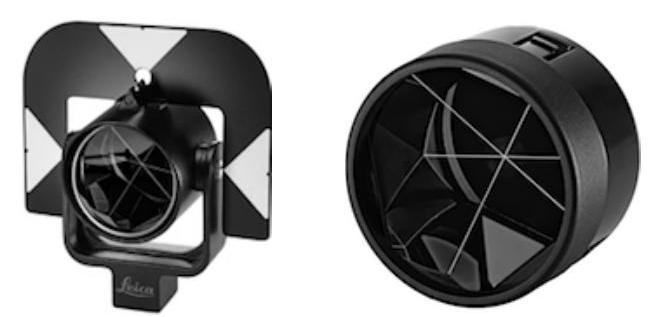
\includegraphics[width=.8\textwidth]{2024_12_07_51b7f57c7f055c2d8d29g-04}
        \caption{Vue externe et détail de la zone en coin de cube d'un prisme optique rétro-réfléchissant}
    \end{subfigure}%
    ~ 
    \begin{subfigure}[t]{0.5\textwidth}
        \centering
        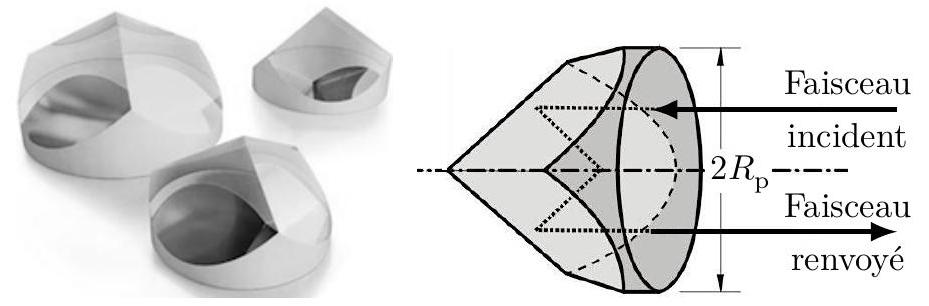
\includegraphics[width=.8\textwidth]{2024_12_07_51b7f57c7f055c2d8d29g-04(1)}
        \caption{Vue générale d'un coin de cube et trajectoire du faisceau laser dans le verre dans le cas d'une incidence normale}
    \end{subfigure}
    %Figure 5 \\
    \caption{Prisme optique rétro-réfléchissant : photographie et principe du renvoi du faisceau laser \label{CCS_MP_2017:fig_05}}
\end{figure*}




On limite l'étude au cas particulier de l'évolution du faisceau laser dans un plan.\\

%Q 5. 
\question{\label{CCS_MP_2017:q_05}Répondre à cette question exclusivement sur la figure A du document réponse. Tracer, dans la configuration proposée (angle d'incidence $i=15^{\circ}$ ) et en justifiant les constructions dans la zone prévue, la trajectoire du faisceau laser à l'intérieur ainsi qu'en sortie du prisme optique rétro-réfléchissant.}
\ifprof
\begin{corrige}
\end{corrige}
\else
\fi

L'utilisation du tachéomètre améliore la qualité des mesures topographiques qui peuvent être par ailleurs réalisées par un seul opérateur après placement du prisme optique rétro-réfléchissant au point à mesurer. La forme de la mesure reste cependant inchangée : l'appareil de mesure, très lourd, est mobile et la cible est fixe.\\
Afin d'améliorer grandement le confort de l'opérateur, il est nécessaire de changer le principe de la mesure en considérant un prisme optique rétro-réfléchissant mobile et un tachéomètre motorisé pouvant suivre automatiquement la cible: c'est le principe d'une station totale, étudiée dans la partie suivante.

